%% LyX 2.2.3 created this file.  For more info, see http://www.lyx.org/.
%% Do not edit unless you really know what you are doing.
\documentclass[ruled]{article}
\usepackage{courier}
\usepackage[T1]{fontenc}
\usepackage[latin9]{inputenc}
\usepackage[letterpaper]{geometry}
\geometry{verbose}
\usepackage{color}
\usepackage{url}
\usepackage{algorithm2e}
\usepackage{amsmath}
\usepackage{amssymb}
\usepackage{titlesec}
\usepackage{graphicx}
\usepackage[export]{adjustbox}
\graphicspath{ {./images/} }
\usepackage{listings}
\usepackage{pdfpages}
\usepackage[unicode=true,
 bookmarks=false,
 breaklinks=false,pdfborder={0 0 1},backref=section,colorlinks=true]
 {hyperref}

\makeatletter

%%%%%%%%%%%%%%%%%%%%%%%%%%%%%% LyX specific LaTeX commands.
\providecommand{\LyX}{\texorpdfstring%
  {L\kern-.1667em\lower.25em\hbox{Y}\kern-.125emX\@}
  {LyX}}
%% Special footnote code from the package 'stblftnt.sty'
%% Author: Robin Fairbairns -- Last revised Dec 13 1996
\let\SF@@footnote\footnote
\def\footnote{\ifx\protect\@typeset@protect
    \expandafter\SF@@footnote
  \else
    \expandafter\SF@gobble@opt
  \fi
}
\expandafter\def\csname SF@gobble@opt \endcsname{\@ifnextchar[%]
  \SF@gobble@twobracket
  \@gobble
}
\edef\SF@gobble@opt{\noexpand\protect
  \expandafter\noexpand\csname SF@gobble@opt \endcsname}
\def\SF@gobble@twobracket[#1]#2{}

\@ifundefined{date}{}{\date{}}
%%%%%%%%%%%%%%%%%%%%%%%%%%%%%% User specified LaTeX commands.
\definecolor{mygreen}{rgb}{0,0.6,0}
\definecolor{mygray}{rgb}{0.5,0.5,0.5}
\definecolor{mymauve}{rgb}{0.58,0,0.82}

\makeatother

\usepackage{listings}
\lstset{backgroundcolor={\color{white}},
basicstyle={\footnotesize\ttfamily},
breakatwhitespace=false,
breaklines=true,
captionpos=b,
commentstyle={\color{mygreen}},
deletekeywords={...},
escapeinside={\%*}{*)},
extendedchars=true,
frame=shadowbox,
keepspaces=true,
keywordstyle={\color{blue}},
language=Python,
morekeywords={*,...},
numbers=none,
numbersep=5pt,
numberstyle={\tiny\color{mygray}},
rulecolor={\color{black}},
showspaces=false,
showstringspaces=false,
showtabs=false,
stepnumber=1,
stringstyle={\color{mymauve}},
tabsize=2}
\begin{document}
\global\long\def\reals{\mathbf{R}}
 \global\long\def\integers{\mathbf{Z}}
\global\long\def\naturals{\mathbf{N}}
 \global\long\def\rationals{\mathbf{Q}}
\global\long\def\ca{\mathcal{A}}
\global\long\def\cb{\mathcal{B}}
 \global\long\def\cc{\mathcal{C}}
 \global\long\def\cd{\mathcal{D}}
\global\long\def\ce{\mathcal{E}}
\global\long\def\cf{\mathcal{F}}
\global\long\def\cg{\mathcal{G}}
\global\long\def\ch{\mathcal{H}}
\global\long\def\ci{\mathcal{I}}
\global\long\def\cj{\mathcal{J}}
\global\long\def\ck{\mathcal{K}}
\global\long\def\cl{\mathcal{L}}
\global\long\def\cm{\mathcal{M}}
\global\long\def\cn{\mathcal{N}}
\global\long\def\co{\mathcal{O}}
\global\long\def\cp{\mathcal{P}}
\global\long\def\cq{\mathcal{Q}}
\global\long\def\calr{\mathcal{R}}
\global\long\def\cs{\mathcal{S}}
\global\long\def\ct{\mathcal{T}}
\global\long\def\cu{\mathcal{U}}
\global\long\def\cv{\mathcal{V}}
\global\long\def\cw{\mathcal{W}}
\global\long\def\cx{\mathcal{X}}
\global\long\def\cy{\mathcal{Y}}
\global\long\def\cz{\mathcal{Z}}
\global\long\def\ind#1{1(#1)}
\global\long\def\pr{\mathbb{P}}

\global\long\def\ex{\mathbb{E}}
\global\long\def\var{\textrm{Var}}
\global\long\def\cov{\textrm{Cov}}
\global\long\def\sgn{\textrm{sgn}}
\global\long\def\sign{\textrm{sign}}
\global\long\def\kl{\textrm{KL}}
\global\long\def\law{\mathcal{L}}
\global\long\def\eps{\varepsilon}
\global\long\def\convd{\stackrel{d}{\to}}
\global\long\def\eqd{\stackrel{d}{=}}
\global\long\def\del{\nabla}
\global\long\def\loss{\ell}
\global\long\def\tr{\operatorname{tr}}
\global\long\def\trace{\operatorname{trace}}
\global\long\def\diag{\text{diag}}
\global\long\def\rank{\text{rank}}
\global\long\def\linspan{\text{span}}
\global\long\def\proj{\text{Proj}}
\global\long\def\argmax{\operatornamewithlimits{arg\, max}}
\global\long\def\argmin{\operatornamewithlimits{arg\, min}}
\global\long\def\bfx{\mathbf{x}}
\global\long\def\bfy{\mathbf{y}}
\global\long\def\bfl{\mathbf{\lambda}}
\global\long\def\bfm{\mathbf{\mu}}
\global\long\def\calL{\mathcal{L}}
\global\long\def\vw{\boldsymbol{w}}
\global\long\def\vx{\boldsymbol{x}}
\global\long\def\vxi{\boldsymbol{\xi}}
\global\long\def\valpha{\boldsymbol{\alpha}}
\global\long\def\vbeta{\boldsymbol{\beta}}
\global\long\def\vsigma{\boldsymbol{\sigma}}
\global\long\def\vmu{\boldsymbol{\mu}}
\global\long\def\vtheta{\boldsymbol{\theta}}
\global\long\def\vd{\boldsymbol{d}}
\global\long\def\vs{\boldsymbol{s}}
\global\long\def\vt{\boldsymbol{t}}
\global\long\def\vh{\boldsymbol{h}}
\global\long\def\ve{\boldsymbol{e}}
\global\long\def\vf{\boldsymbol{f}}
\global\long\def\vg{\boldsymbol{g}}
\global\long\def\vz{\boldsymbol{z}}
\global\long\def\vk{\boldsymbol{k}}
\global\long\def\va{\boldsymbol{a}}
\global\long\def\vb{\boldsymbol{b}}
\global\long\def\vv{\boldsymbol{v}}
\global\long\def\vy{\boldsymbol{y}}



\title{Machine Learning and Computational Statistics\\
Gradient Descent}
\author{Nhung Le}

\maketitle
\textbf{Note}: This document consists of concepts and exercises related to Gradient Descent.

\section{Concepts}
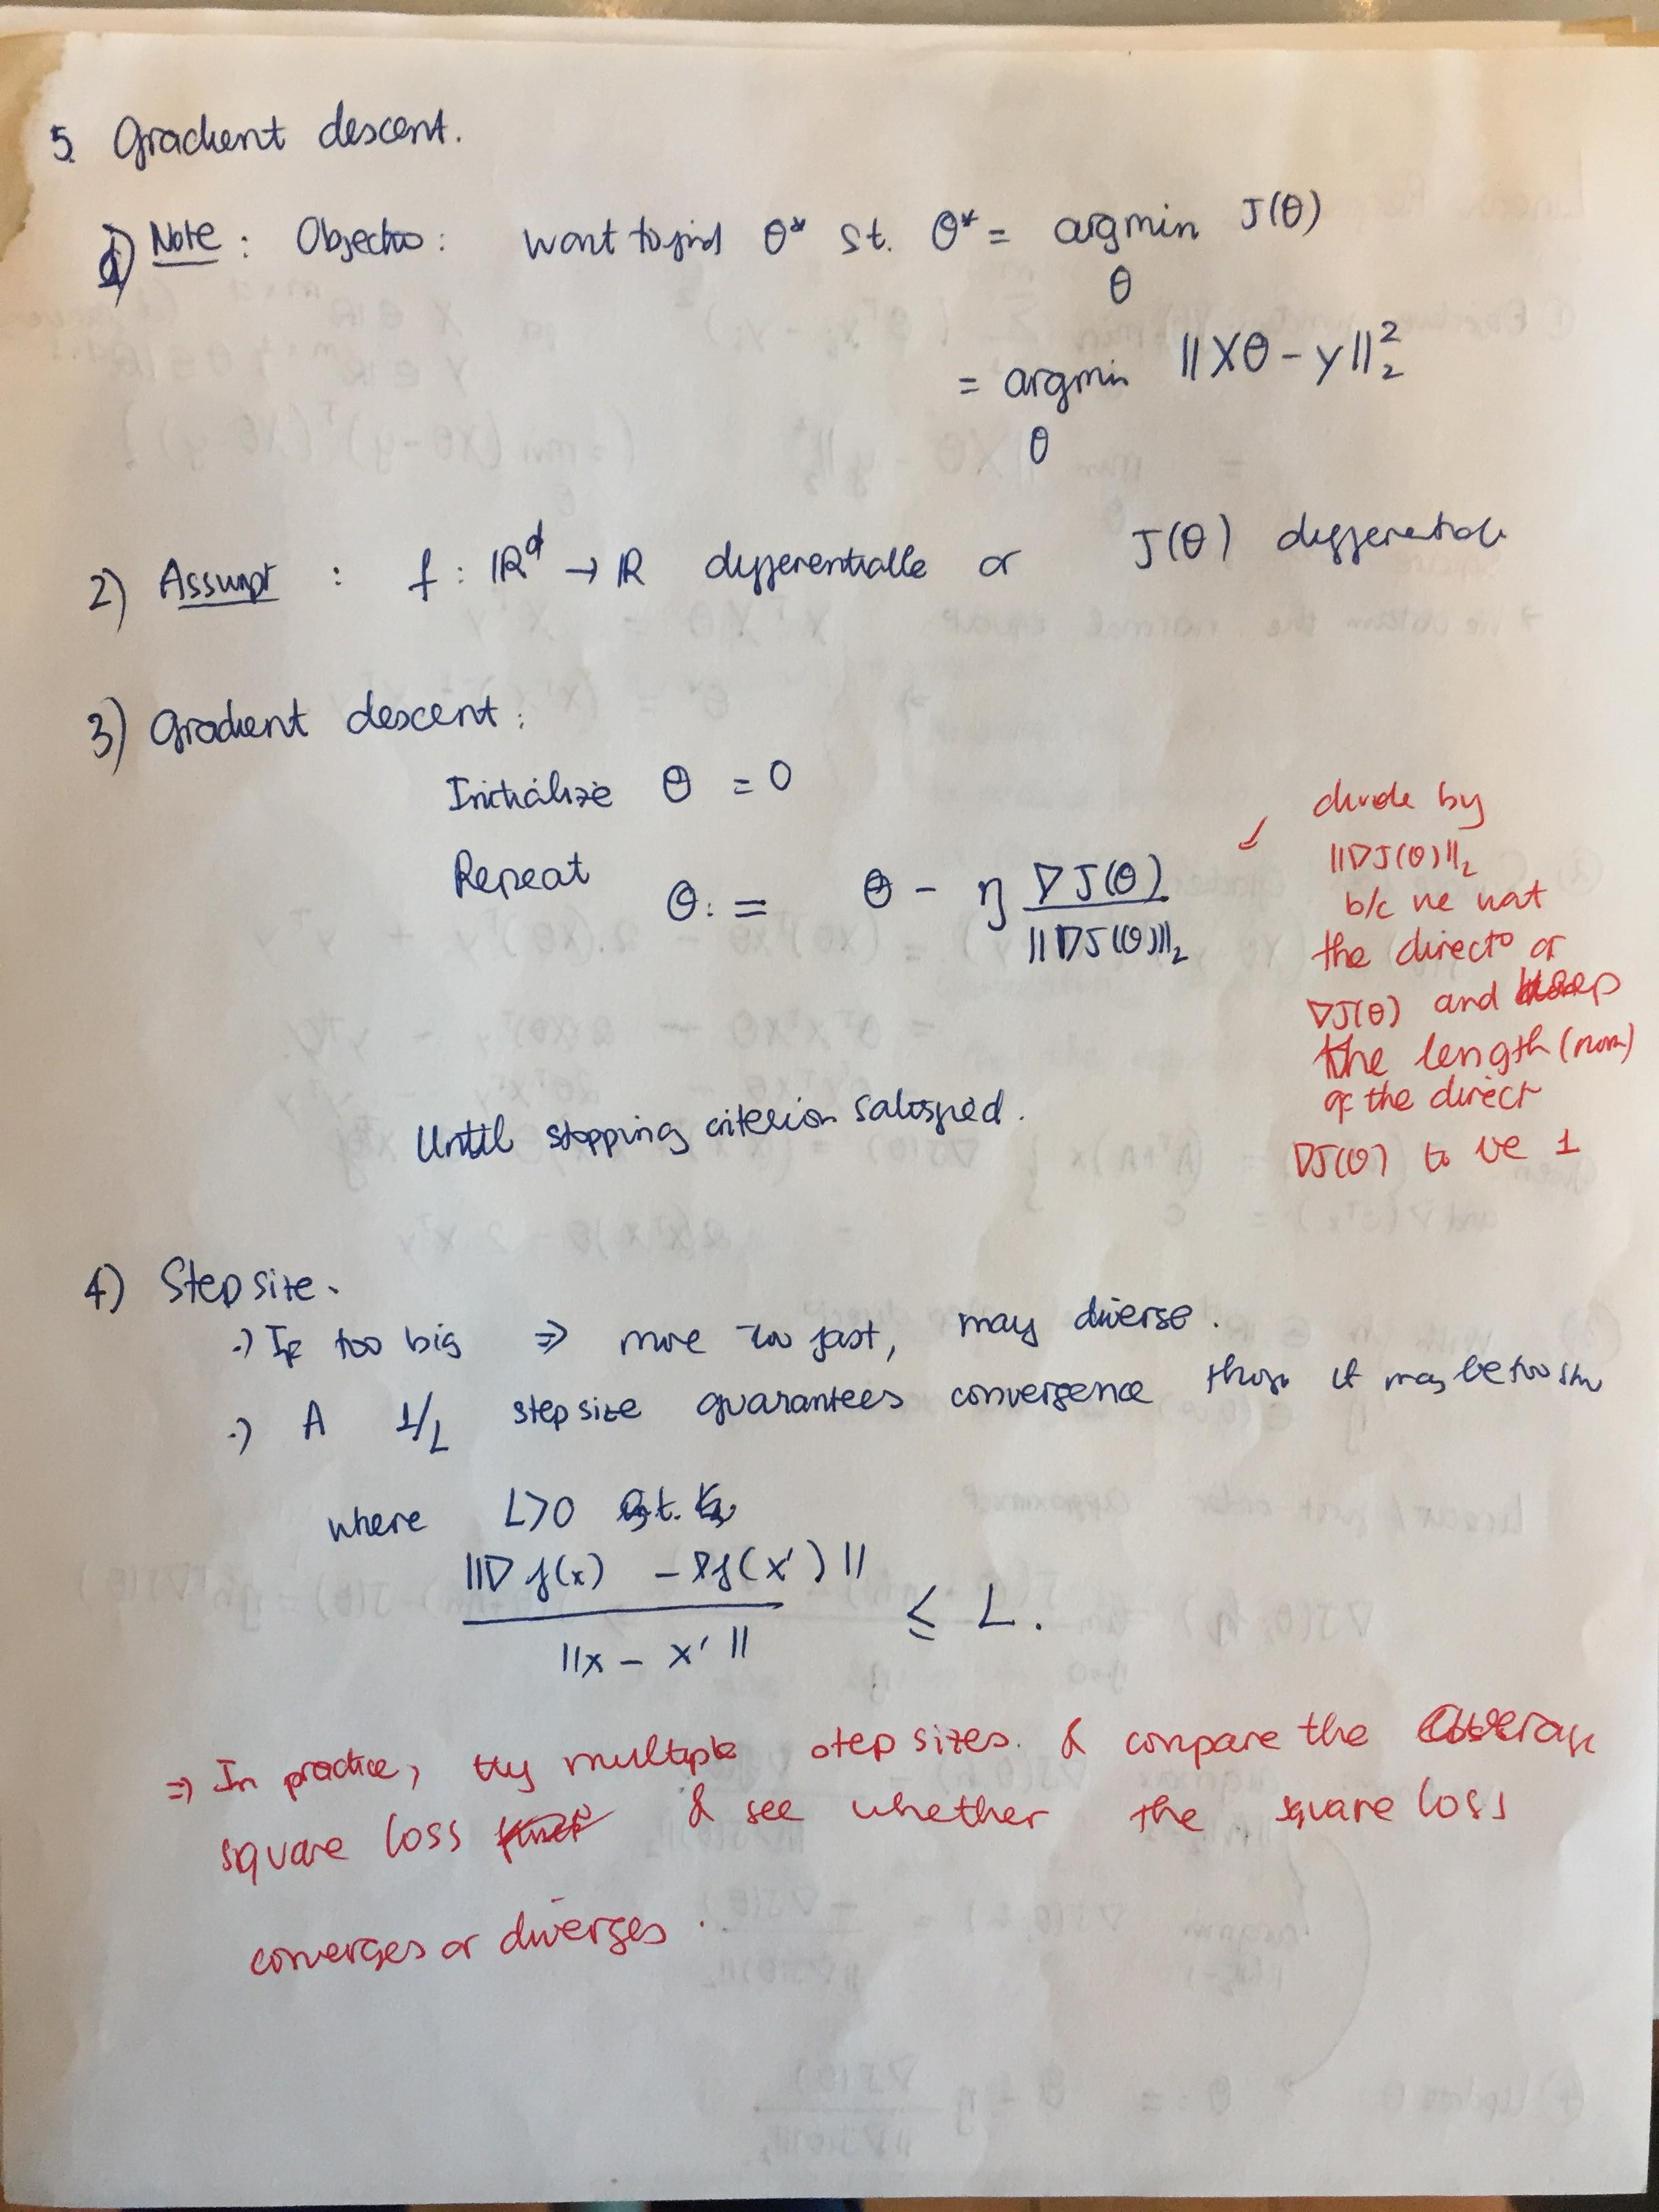
\includegraphics[max size={\textwidth}{\textheight}]{GradDesc1.jpg} \\

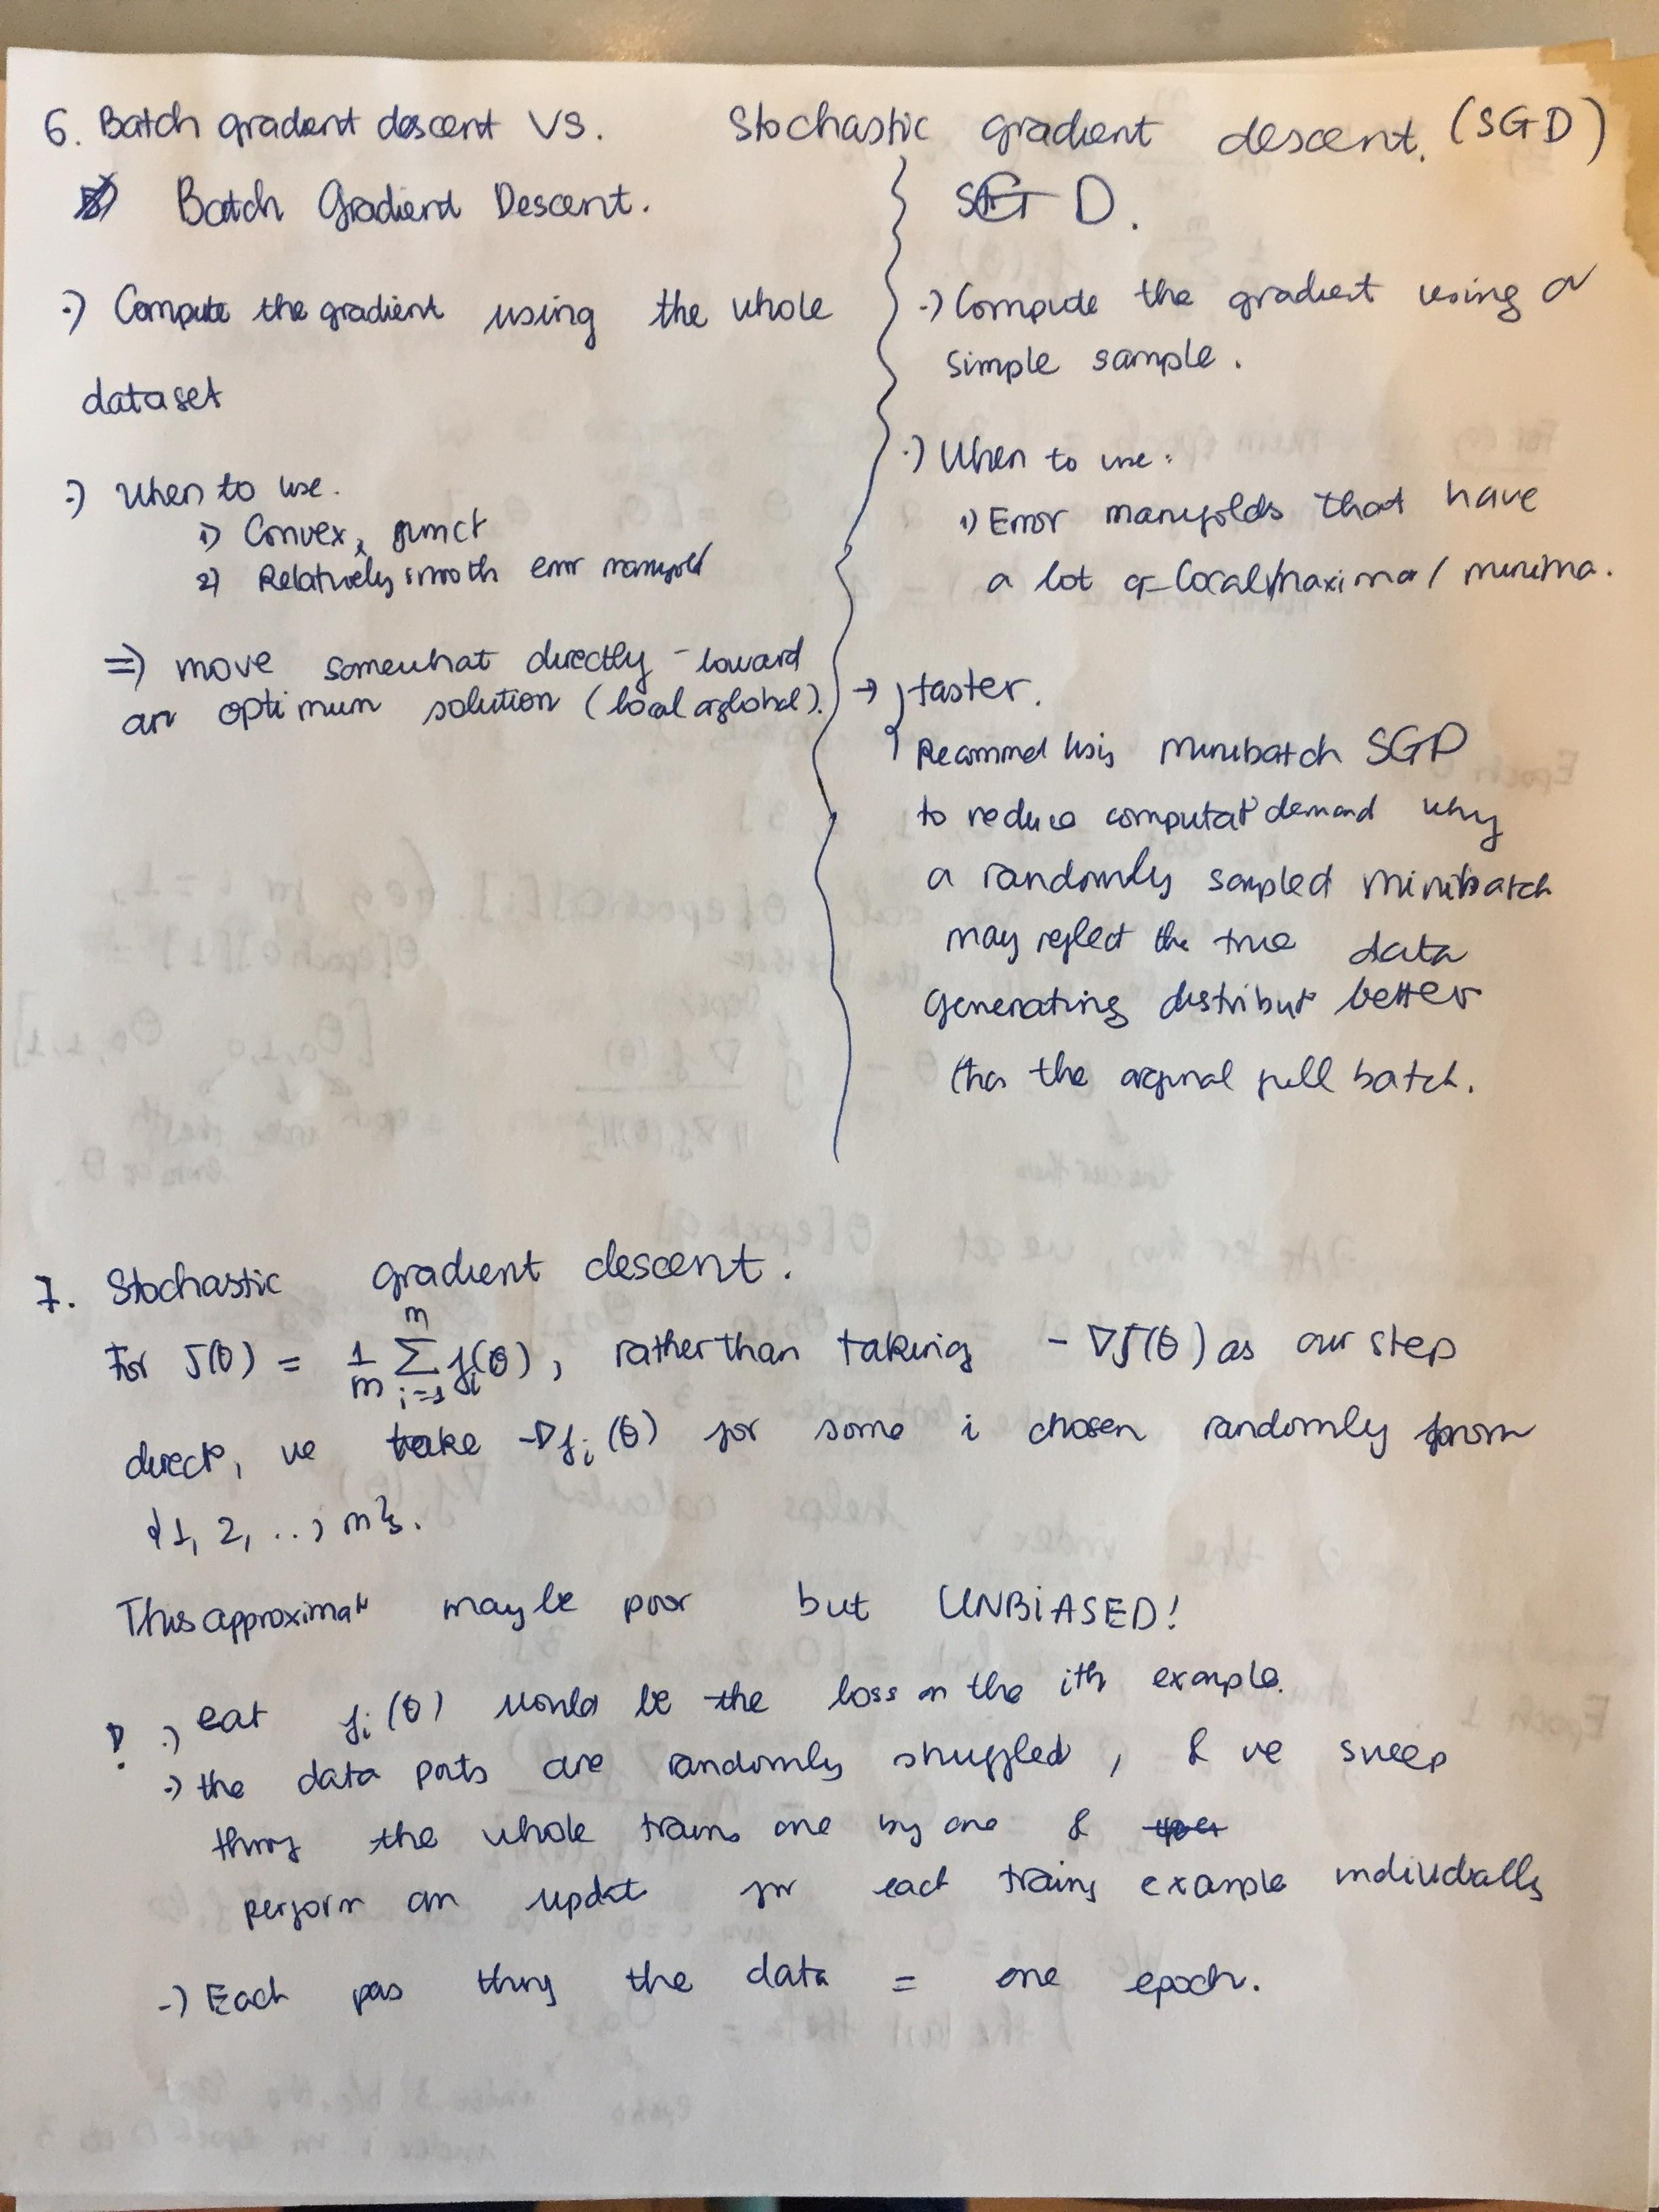
\includegraphics[max size={\textwidth}{\textheight}]{GradDesc2.jpg} \\
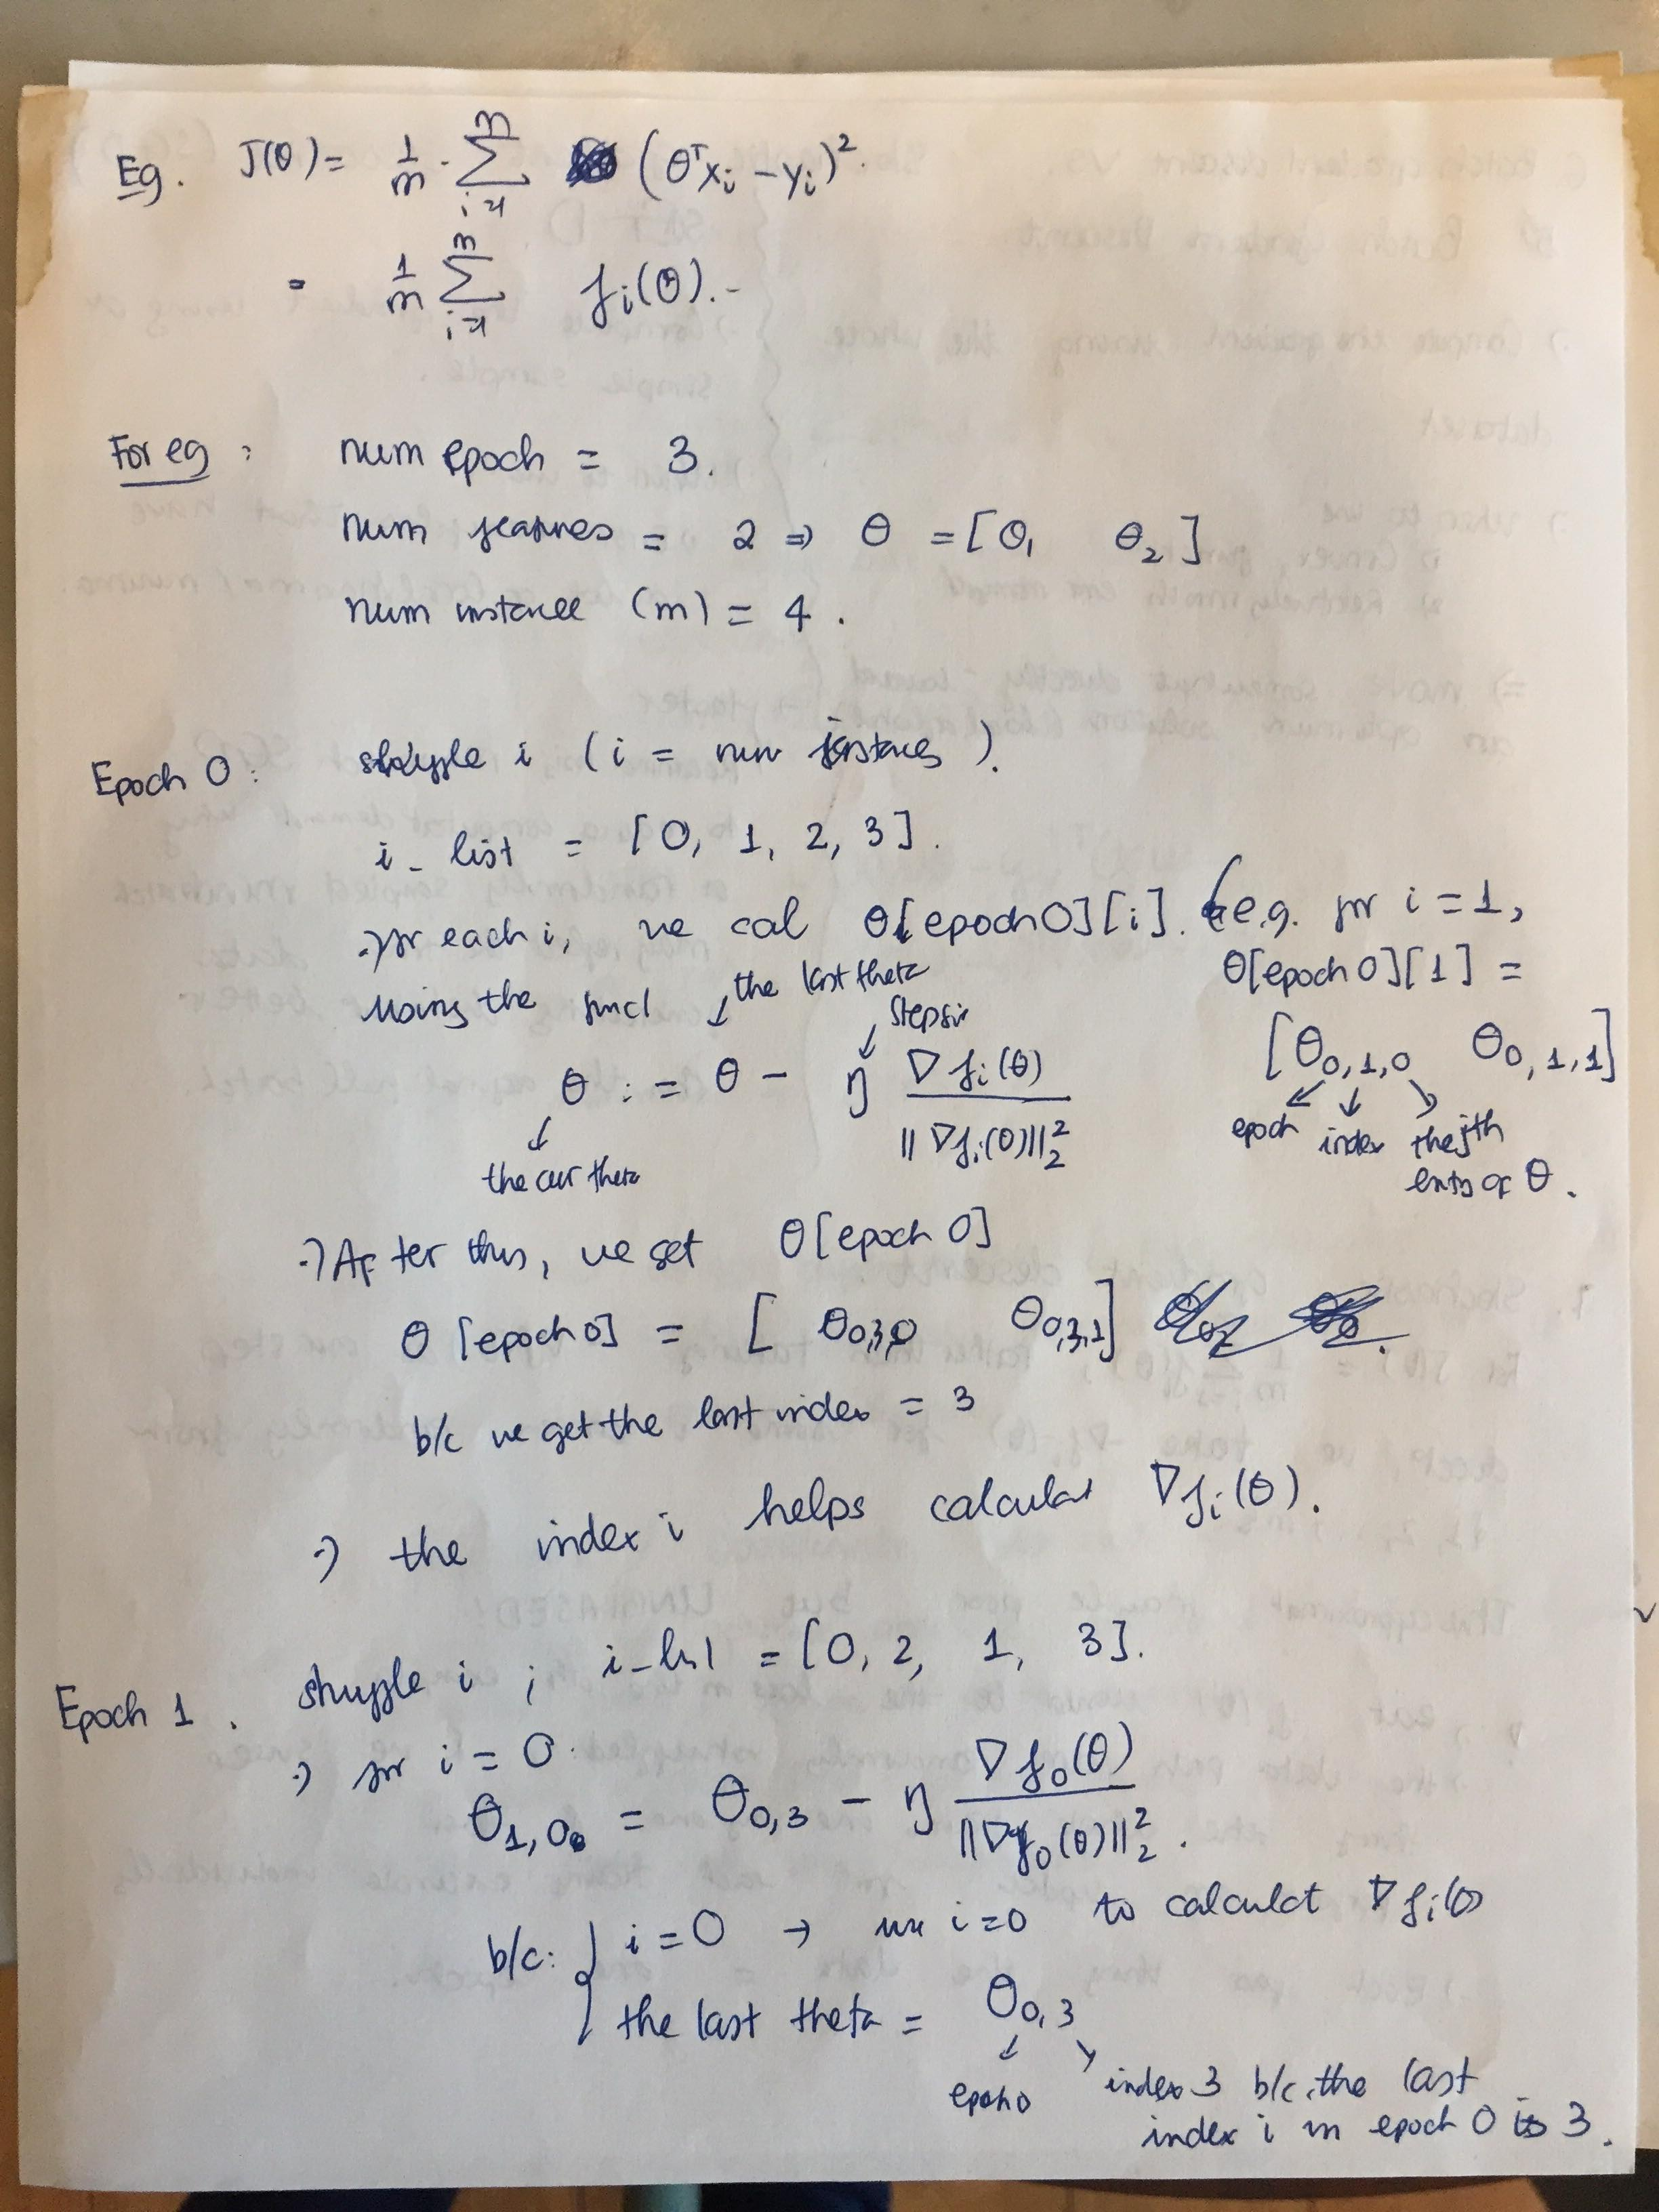
\includegraphics[max size={\textwidth}{\textheight}]{GradDesc3.jpg} \\

\section{Linear Regression and Gradient Descent}

\subsection{Feature Normalization}

When feature values differ greatly, we can get much slower rates of
convergence of gradient-based algorithms. Furthermore, when we start
using regularization (introduced in a later problem), features with
larger values are treated as ``more important'', which is not usually
what you want.  One common approach to feature normalization is perform
an affine transformation (i.e. shift and rescale) on each feature
so that all feature values in the training set are in $[0,1]$. Each
feature gets its own transformation. We then apply the same transformations
to each feature on the test\footnote{Throughout this assignment we refer to the ``test'' set. It may
be more appropriate to call this set the ``validation'' set, as
it will be a set of data on which we compare the performance of multiple
models. Typically a test set is only used once, to assess the performance
of the model that performed best on the validation set.} set. It's important that the transformation is ``learned'' on the
training set, and then applied to the test set. It is possible that
some transformed test set values will lie outside the $[0,1]$ interval.

\subsection{Gradient Descent Setup}

In linear regression, we consider the hypothesis space of linear functions
$h_{\theta}:\reals^{d}\to\reals$, where
\[
h_{\theta}(x)=\theta^{T}x,
\]
for $\theta,x\in\reals^{d}$, and we choose $\theta$ that minimizes
the following ``average square loss'' objective function: 
\[
J(\theta)=\frac{1}{m}\sum_{i=1}^{m}\left(h_{\theta}(x_{i})-y_{i}\right)^{2},
\]
where $(x_{1},y_{1}),\ldots,(x_{m},y_{m})\in\reals^{d}\times\reals$
is our training data.

While this formulation of linear regression is very convenient, it's
more standard to use a hypothesis space of ``affine'' functions:
\[
h_{\theta,b}(x)=\theta^{T}x+b,
\]
which allows a ``bias'' or nonzero intercept term. The standard
way to achieve this, while still maintaining the convenience of the
first representation, is to add an extra dimension to $x$ that is
always a fixed value, such as 1. You should convince yourself that
this is equivalent. We'll assume this representation, and thus we'll
actually take $\theta,x\in\reals^{d+1}$.
\begin{enumerate}
\item Let $X\in\reals^{m\times\left(d+1\right)}$ be the \textbf{design
matrix}, where the $i$'th row of $X$ is $x_{i}$. Let $y=\left(y_{1},\ldots,y_{m}\right)^{T}\in\reals^{m\times1}$
be the ``response''. The objective function $J(\theta)$:

$J(\theta) = \frac{1}{m} (X\theta - y)^T \cdot (X\theta - y)$ 


\item The gradient of $J$: 

$\nabla_{\theta} J(\theta)= \frac{2}{m}X^T(X\theta - y)$

\item In our search for a $\theta$ that minimizes $J$, suppose we take
a step from $\theta$ to $\theta+\eta h$, where $h\in\reals^{d+1}$
is the ``step direction'' (recall, this is not necessarily a unit
vector) and $\eta\in(0,\infty)$ is the ``step size'' (note that
this is not the actual length of the step, which is $\eta\|h\|$).
An approximate expression for the change
in objective function value $J(\theta+\eta h)-J(\theta)$. 

$J(\theta+\eta h)-J(\theta) \approx \nabla_{\theta} J(\theta)^T (\theta + \eta h - \theta) = \eta  \nabla_{\theta} J(\theta)^T h$

\item The expression for updating $\theta$ in the gradient descent
algorithm. Let $\eta$ be the step size.

$\theta_{n+1} = \theta_{n} - \eta  \nabla J(\theta_{n})$

\item Compute $J(\theta)$ for a given $\theta$. \footnote{Refer to function \texttt{ compute\_square\_loss(X, y, theta)} Q2.2 HW1 2019}

\item compute
$\del_{\theta}J(\theta)$ \footnote{Refer to \texttt{compute\_square\_loss\_gradient} Q2.2 HW1 2019} 
\end{enumerate}



\subsection{Gradient Checker}

\noindent For many optimization problems, coding up the gradient correctly
can be tricky. Luckily, there is a nice way to numerically check the
gradient calculation. If $J:\reals^{d}\to\reals$ is differentiable,
then for any vector $h\in\reals^{d}$, the directional derivative
of $J$ at $\theta$ in the direction $h$ is given by\footnote{Of course, it is also given by the more standard definition of directional
derivative, $\lim_{\eps\to0}\frac{1}{\eps}\left[J(\theta+\eps h)-J(\theta)\right]$.
The form given gives a better approximation to the derivative when
we are using small (but not infinitesimally small) $\eps$.}
\[
\lim_{\eps\to0}\frac{J(\theta+\eps h)-J(\theta-\eps h)}{2\epsilon}.
\]
We can approximate this directional derivative by choosing a small
value of $\eps>0$ and evaluating the quotient above. We can get an
approximation to the gradient by approximating the directional derivatives
in each coordinate direction and putting them together into a vector.
In other words, take $h=\left(1,0,0,\ldots,0\right)$ to get the first
component of the gradient. Then take $h=(0,1,0,\ldots,0)$ to get
the second component. And so on. See \url{http://ufldl.stanford.edu/wiki/index.php/Gradient_checking_and_advanced_optimization}
for details. 

\subsection{Batch Gradient Descent\protect\footnote{Sometimes people say ``batch gradient descent'' or ``full batch
gradient descent'' to mean gradient descent, defined as we discussed
in class. They do this to distinguish it from stochastic gradient
descent and minibatch gradient descent, which they probably use as
their default.}}

\begin{enumerate}
\item Batch Gradient Descent \footnote{Refer to Q2.4 HW1-2019}

\item Step size: The step size affects whether and how fast gradient descent converges (i.e., if step size is too large, gradient descent may not converge\footnote{For the mathematically inclined, there is a theorem that if the objective
function is convex and differentiable, and the gradient of the objective
is Lipschitz continuous with constant $L>0$, then gradient descent
converges for fixed steps of size $1/L$ or smaller. See \url{https://www.cs.cmu.edu/~ggordon/10725-F12/scribes/10725_Lecture5.pdf},
Theorem 5.1.}. 
As shown below, when the step size is large (e.g., 0.5) the loss oscilates around a lot but does tend to become smaller over time. When the step size is smaller (e.g., 0.05, 0.01), the loss converges faster, especially when we get closer to the optimal point \footnote{Refer to HW1-2019} 

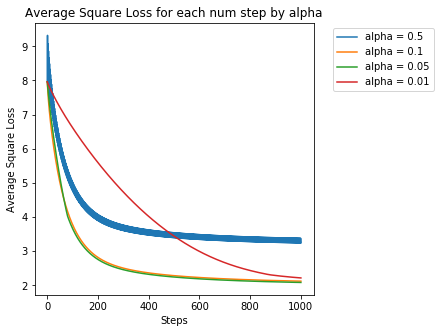
\includegraphics{pic1} 

\end{enumerate}

\section{Ridge Regression (i.e. Linear Regression with $\ell_{2}$ regularization) and Gradient Descent}

When we have a large number of features compared to instances, regularization
can help control overfitting. Ridge regression is linear regression
with $\ell_{2}$ regularization. The regularization term is sometimes
called a penalty term. The objective function for ridge regression
is
\[
J(\theta)=\frac{1}{m}\sum_{i=1}^{m}\left(h_{\theta}(x_{i})-y_{i}\right)^{2}+\lambda\theta^{T}\theta,
\]
where $\lambda$ is the regularization parameter, which controls the
degree of regularization. Note that the bias parameter is being regularized
as well. We will address that below.
\begin{enumerate}
\item  The gradient of $J(\theta)$

$ \nabla_{theta} J(\theta) = \frac{2}{m} X^T (X \theta - y) + 2 \lambda \theta$ 

\item Updating $\theta$ in the gradient descent algorithm

$\theta_{n+1} = \theta_{n} - \eta  [\frac{2}{m} X^T (X \theta - y) + 2 \lambda \theta] $


\item Compute regularized square loss gradient \footnote{Refer to \texttt{\_regularized\_square\_loss\_gradient} function from HW1-2019}

\item Compute gradient descent \footnote{Refer to  \texttt{regularized\_grad\_descent.} from HW1 - 2019 }

\item For regression problems, we may prefer to leave the bias term unregularized.
One approach is to change $J(\theta)$ so that the bias is separated
out from the other parameters and left unregularized. Another approach
that can achieve approximately the same thing is to use a very large
number $B$, rather than $1$, for the extra bias dimension. When B is really large, it means the corresponding coefficient is small, leading to smaller effect of the intercept on regularization. Thus, the bias term is un-regularized. \\

Suppose we have an affine function $f(x) = \theta_0 B + \theta^Tx $ . where we have separated out $B$ from the vector $x$. If we increase $B$, the corresponding coefficient $\theta_0$ will have to decrease by the same
factor to end up with the same function f. A smaller coefficient  $\theta_0$ incurs less regularization
penalty. As $ B \rightarrow \infty, B_0 \rightarrow 0$ and the regularization effect approaches 0


\item Now fix $B=1$, find the $\theta_{\lambda}^{*}$ that minimizes $J(\theta)$
over a range of $\lambda$. The goal is to find $\lambda$
that gives the minimum average square loss on the test set. It's hard to predict what $\lambda$
that will be, so you should start your search very broadly, looking
over several orders of magnitude. For example, $\lambda\in\left\{ 10^{-7},10^{-5},10^{-3},10^{-1},1,10,100\right\} $.
Once you find a range that works better, keep zooming in. You may
want to have $\log(\lambda)$ on the $x$-axis rather than $\lambda$.
{[}If you like, you may use sklearn to help with the hyperparameter
search.{]} 

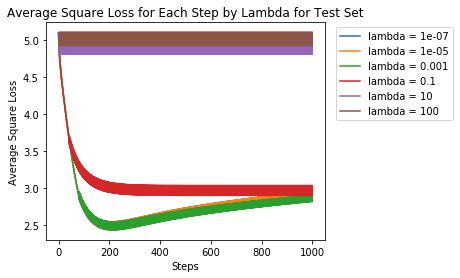
\includegraphics{pic2}
\end{enumerate}

\section{Stochastic Gradient Descent}

\noindent When the training data set is very large, evaluating the
gradient of the objective function can take a long time, since it
requires looking at each training example to take a single gradient
step. When the objective function takes the form of an average of
many values, such as
\[
J(\theta)=\frac{1}{m}\sum_{i=1}^{m}f_{i}(\theta)
\]
 (as it does in the empirical risk), stochastic gradient descent (SGD)
can be very effective. In SGD, rather than taking $-\del J(\theta)$
as our step direction, we take $-\del f_{i}(\theta)$ for some $i$
chosen uniformly at random from $\{1,\ldots,m\}$. The approximation
is poor, but we will show it is unbiased. 

\noindent In machine learning applications, each $f_{i}(\theta)$
would be the loss on the $i$th example (and of course we'd typically
write $n$ instead of $m$, for the number of training points). In
practical implementations for ML, the data points are \textbf{randomly
shuffled}, and then we sweep through the whole training set one by
one, and perform an update for each training example individually.
One pass through the data is called an \textbf{epoch}. Note that each
epoch of SGD touches as much data as a single step of batch gradient
descent. You can use the same ordering for each epoch, though optionally
you could investigate whether reshuffling after each epoch affects
the convergence speed. 
\begin{enumerate}
\item The objective function 
\[
J(\theta)=\frac{1}{m}\sum_{i=1}^{m}\left(h_{\theta}(x_{i})-y_{i}\right)^{2}+\lambda\theta^{T}\theta
\]
can be written in the form $J(\theta)=\frac{1}{m}\sum_{i=1}^{m}f_{i}(\theta)$ with $f_{i}(\theta)$ to be: 

$f_{i}(\theta) = (h_{\theta}(x_{i})-y_{i})^2 + \lambda\theta^{T}\theta$

\item We can easily show that the stochastic gradient $\del f_{i}(\theta)$, for $i$
chosen uniformly at random from $\{1,\ldots,m\}$, is an \textbf{unbiased
estimator} of $\del J(\theta)$. In other words, $\ex\left[\del f_{i}(\theta)\right]=\del J(\theta)$
for any $\theta$. 

\item The update rule for $\theta$ in SGD for the ridge
regression objective function. \\
$\nabla f_i (\theta) = 2 (h_{\theta} x_i - y_i ) x_i + 2 \lambda x_i =  2 (\theta_i^T x_i - y_i ) x_i + 2 \lambda x_i $

$\theta_{i+1} = \theta_i - \eta \nabla f_i(\theta) = \theta_i - \eta  [2 (\theta_i^T x_i - y_i ) x_i + 2 \lambda x_i]$

\item Implement Stochastic Grad Descent \footnote{Refer to \texttt{stochastic\_grad\_descent} from HW1 - 2019} 

\item Use SGD to find $\theta_{\lambda}^{*}$ that minimizes the ridge regression
objective for the $\lambda$ and $B$ selected in the previous
problem. 

\item Step Size: Try step sizes that decrease with the step number according
to the following schedules: $\eta_{t}=\frac{C}{t}$ and $\eta_{t}=\frac{C}{\sqrt{t}}$, $C \leq 1$. Please include $C = 0.1$ in your submissions. 


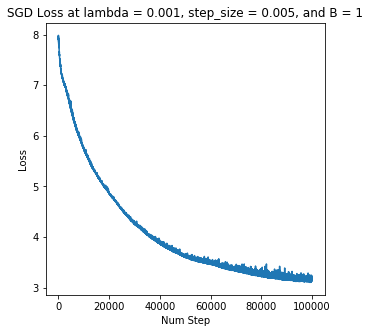
\includegraphics{pic3}\\
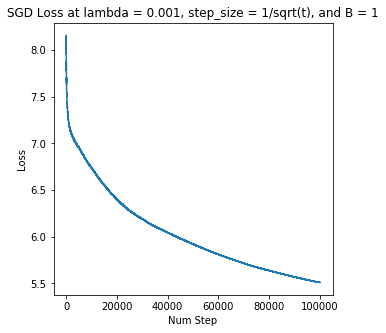
\includegraphics{pic4}\\
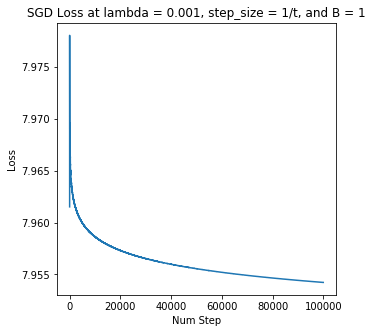
\includegraphics{pic5}\\

As shown above, the min loss is 3.131 achieve when step size is 0.05. \\
The $\theta$ is:
[-1.341736    0.74105522  1.15087591  2.26252857 -2.47698603 -0.78870877
 -0.66170294 -0.66170294  0.69995027  1.00150192  1.35592862  0.20464685
 -1.49757454 -2.45934331  1.25037301  1.87837869  0.75761022  0.60828829
 -0.0038115  -0.0038115  -0.0038115   0.05589895  0.05589895  0.05589895
  0.07780999  0.07780999  0.07780999  0.0886481   0.0886481   0.0886481
  0.09487685  0.09487685  0.09487685 -0.06370046 -0.06370046 -0.06370046
  0.11790856  0.11790856  0.11790856  0.11413693  0.11413693  0.11413693
  0.11280427  0.11280427  0.11280427  0.11218991  0.11218991  0.11218991
 -1.33892822]


Some things to note: 
\begin{itemize}
\item In this case we are investigating the convergence rate of
the optimization algorithm with different step size schedules, thus
we're interested in the value of the objective function, which includes
the regularization term.
\item Sometimes the initial step size ($C$
for $C/t$ and $C/\sqrt{t}$) is too aggressive and will get you into
a part of parameter space from which you can't recover. Try reducing $C$ to counter this problem. 
\item As we'll learn in an upcoming lecture, SGD
convergence is much slower than GD once we get close to the minimizer.
(Remember, the SGD step directions are very noisy versions of the
GD step direction). If you look at the objective function values on
a logarithmic scale, it may look like SGD will never find objective
values that are as low as GD gets. In terminology we'll learn in Lecture
2, GD has much smaller ``optimization error'' than SGD. However,
this difference in optimization error is usually dominated by other
sources of error (estimation error and approximation error). Moreover,
for very large datasets, SGD (or minibatch GD) is much faster (by
wall-clock time) than GD to reach a point that's close {[}enough{]}
to the minimizer. 
\item (Optional) There is another variant of SGD, sometimes called \textbf{averaged SGD}, in which rather than using the last parameter value we visit, say $\theta^T$, we use the average of all parameter values we visit along the optimization path: $\theta = \frac{1}{T}\sum_{t=1}^{T}\theta^t$, where $T$ is total number of steps taken. Try this approach\footnote{Some theory for averaged SGD is given on page $191$ of \href{http://www.cs.huji.ac.il/~shais/UnderstandingMachineLearning/understanding-machine-learning-theory-algorithms.pdf}{Understanding Machine Learning: From Theory to Algorithms}. Refer to page 195 of the same book for other averaging techniques you can try.} and see how it compares.
\end{itemize}

\item (Optional) Try a stepsize rule of the form $\eta_{t}=\frac{\eta_{0}}{1+\eta_{0}\lambda t}$,
where $\lambda$ is your regularization constant, and $\eta_{0}$
a constant you can choose. How do the results compare?
\end{enumerate}


\end{document}
